\documentclass{article}

\usepackage{fullpage,verbatim,amsmath,graphicx,listings,color}

\newcommand{\HRule}{\rule{\linewidth}{0.5mm}}
\begin{document}

\lstset{
language=Python, 
basicstyle=\scriptsize,
backgroundcolor=\color{white},
showspaces=false,
showstringspaces=false,
showtabs=false,
frame=shadowbox,
tabsize=4,
captionpos=b,
title=\lstname,
breaklines=true,
breakatwhitespace=true}

\begin{titlepage}
 
\begin{center}
 
\textsc{\LARGE Homework 5}\\[1.5cm] 

\textsc{\Large Computational Math}\\[0.5cm]
 
 
\HRule \\[2cm]
 
% Author and supervisor
\begin{minipage}{0.4\textwidth}
\begin{flushleft} \large
\emph{Author:}\\
Mikola Lysenko
\end{flushleft}
\end{minipage}
 
\vfill
 
% Bottom of the page
{\large \today}
 
\end{center}
 
\end{titlepage}


\paragraph{1}

\subparagraph{a}
For the test functions, choose $u,v$ from the space of continuous functions supported on $\Omega$; ie $\text{supp } u \subseteq \Omega$.  Now for any solution $u$ with test function $v$ we must have:
\[ \int \limits_{\Omega} - u_{xx}(x,y) v(x,y) - u_{yy}(x,y) v(x,y) d \Omega = \int \limits_{\Omega} f(x,y) v(x,y) d \Omega \]
Starting on the left hand side, we work term by term:
\begin{eqnarray*}
\int \limits_{-1}^{1} \int \limits_{-1}^{1} -u_{xx}(x,y) v(x,y) dx dy & = &
\int \limits_{-1}^{1} \left( -u_x(x,y) v(x,y) |_{-1}^{1} + \int \limits_{-1}^{1} u_{x}(x,y) v_{x}(x,y) dx \right) dy \\
& = & \int \limits_{\Omega} u_{x}(x,y) v_{x}(x,y) d \Omega \\
& = & p_1(u, v)
\end{eqnarray*}
By symmetry:
\[ p_2(u,v) = \int \limits_{\Omega} u_{yy} v d \Omega = \int \limits_{\Omega} u_{y}(x,y) v_{y}(x,y) d \Omega \]
For the right hand side, we just get:
\[ b(v) = \int \limits_{\Omega} f(x,y) v(x,y) d \Omega \]
And so the weak form of the variational problem is:
\[ p_1(u,v) + p_2(u,v) = b(v) \]

\subparagraph{b}

Let $(x_1, y_1), (x_2, y_2), (x_3, y_3), (x_4, y_4)$ be the nodes of the element, oriented clockwise.  We now solve for $\alpha_1, \alpha_2, \alpha_3, \alpha_4$ for the node $(x_1, y_1)$.  Plugging in values, we get the following linear system:
\begin{eqnarray*}
\alpha_1 + \alpha_2 x_1 + \alpha_3 y_1 + \alpha_4 x_1 y_1 & = & 1 \\
\alpha_1 + \alpha_2 x_2 + \alpha_3 y_2 + \alpha_4 x_1 y_2 & = & 0 \\
\alpha_1 + \alpha_2 x_3 + \alpha_3 y_3 + \alpha_4 x_1 y_3 & = & 0 \\
\alpha_1 + \alpha_2 x_4 + \alpha_3 y_4 + \alpha_4 x_4 y_4 & = & 0
\end{eqnarray*}
For the sake of simplicity, we rewrite the system in matrix form:
\[ M \alpha = c \]
Where $\alpha$ is the vector of coefficients. Since $c$ is a basis vector, the values for $\alpha$ at various nodes are just the corresponding rows of $M^{-1}$.  

Now to construct the matrix equations for this system, we first consider the weak form from part a on a per element basis.  Thus let $\varphi^i, \varphi^j$ be two test functions on a quad element where
\[ \varphi^i(x) = \alpha^i_1 + \alpha^i_2 x + \alpha^i_3 y + \alpha^i_4 x y \]
And:
\[ \varphi^i_{x}(x) = \alpha^i_2 + \alpha^i_4 y \]
To integrate $p_1(\varphi^i, \varphi^j)$, we split the integral into two triangles, indexed by $\Delta(1, 2, 3)$ and $\Delta(1, 3, 4)$, then integrate in barycentric coordinates.  We do this for the first triangle $\Delta(1,2,3)$ now.  Let:
\[ J = \left( \begin{array}{cc}
x_2 - x_1 & y_2 - y_1 \\
x_3 - x_1 & y_3 - y_1
\end{array} \right) \]
And define the affine transformation:
\[ \mathcal{T}(\lambda_1, \lambda_2) = J \left( \begin{array}{c}
\lambda_1 \\
\lambda_2 \\
\end{array} \right) + \left( \begin{array}{c}
x_1 \\
y_1 \\
\end{array} \right) \]
And so we get the following:
\begin{eqnarray*}
\int \limits_{\Delta(1,2,3)} \varphi^i_x(x,y) \varphi^j_x(x,y) d x d y & = & 
\frac{1}{\det J} \int \limits_{0}^{1} \int \limits_{0}^{1- \lambda_2} \varphi^i_{x}(\mathcal{T} (\lambda_1, \lambda_2)) \varphi^j_{x}(\mathcal{T}(\lambda_1, \lambda_2))) d \lambda_1 d \lambda_2  \\
& = & \frac{1}{\det J} \int \limits_{0}^{1} \int \limits_{0}^{1 - \lambda_2}
\alpha^i_2 \alpha^j_2 + (\alpha^i_4 \alpha^j_2  + \alpha^i_2 \alpha^j_4) (J_{2,1} \lambda_1 + J_{2,2} \lambda_2 + y_1) \\
& & \:\:\:\:\:\:\:\:\:\:\:\:\:\: + \:\: \alpha^i_4 \alpha^j_4 (J_{2,1} \lambda_1 + J_{2,2} \lambda_2 + y_1)^2 d \lambda_1 d \lambda_2 
\end{eqnarray*}
To simplify the expression, make the following substitutions:
\begin{eqnarray*}
Q_0 & = & \alpha^i_2 \alpha^j_2 \\
Q_1 & = & \alpha^i_2 \alpha^j_4 + \alpha^i_4 \alpha^j_2 \\
Q_2 & = & \alpha^i_4 \alpha^j_4
\end{eqnarray*}
And so we get the following quantity:
\[ = \frac{1}{2\det J} \left( 
  Q_0 + y_1 \left( Q_1 + y_1 Q_2 \right)
+ \frac{J_{2,1} + J_{2,2}}{3} \left(  
   Q_1 + \left( 2 y_1 + \frac{J_{2,1} + J_{2,2}}{2} \right) Q_2 \right)  - \frac{J_{2,1} J_{2,2} Q_2}{6} \right) \]
We shall call this quantity $T^1_1$, where the upper index denotes the triangle and the lower index denotes the $p_1$ component of the Laplacian, thus we get:
\[ A(\varphi^i, \varphi^j) = p_1(\varphi^i, \varphi^j) + p_2(\varphi^i, \varphi^j) = \sum T^1_1 + T^1_2 + T^2_1 + T^2_2 \]
And so the final matrix is just formed by summing over all such values.  Computing $f$ can be done approximately by sampling at the nodal values.

\subparagraph{c}

Here is the solver I wrote to implement the described method (in Python):

\pagebreak
\lstinputlisting{solver1.py}

And here is the script I wrote to test it on the prescribed problem:

\lstinputlisting{prob1.py}

This is a heatmap plot of the resulting distribution:

\begin{center}
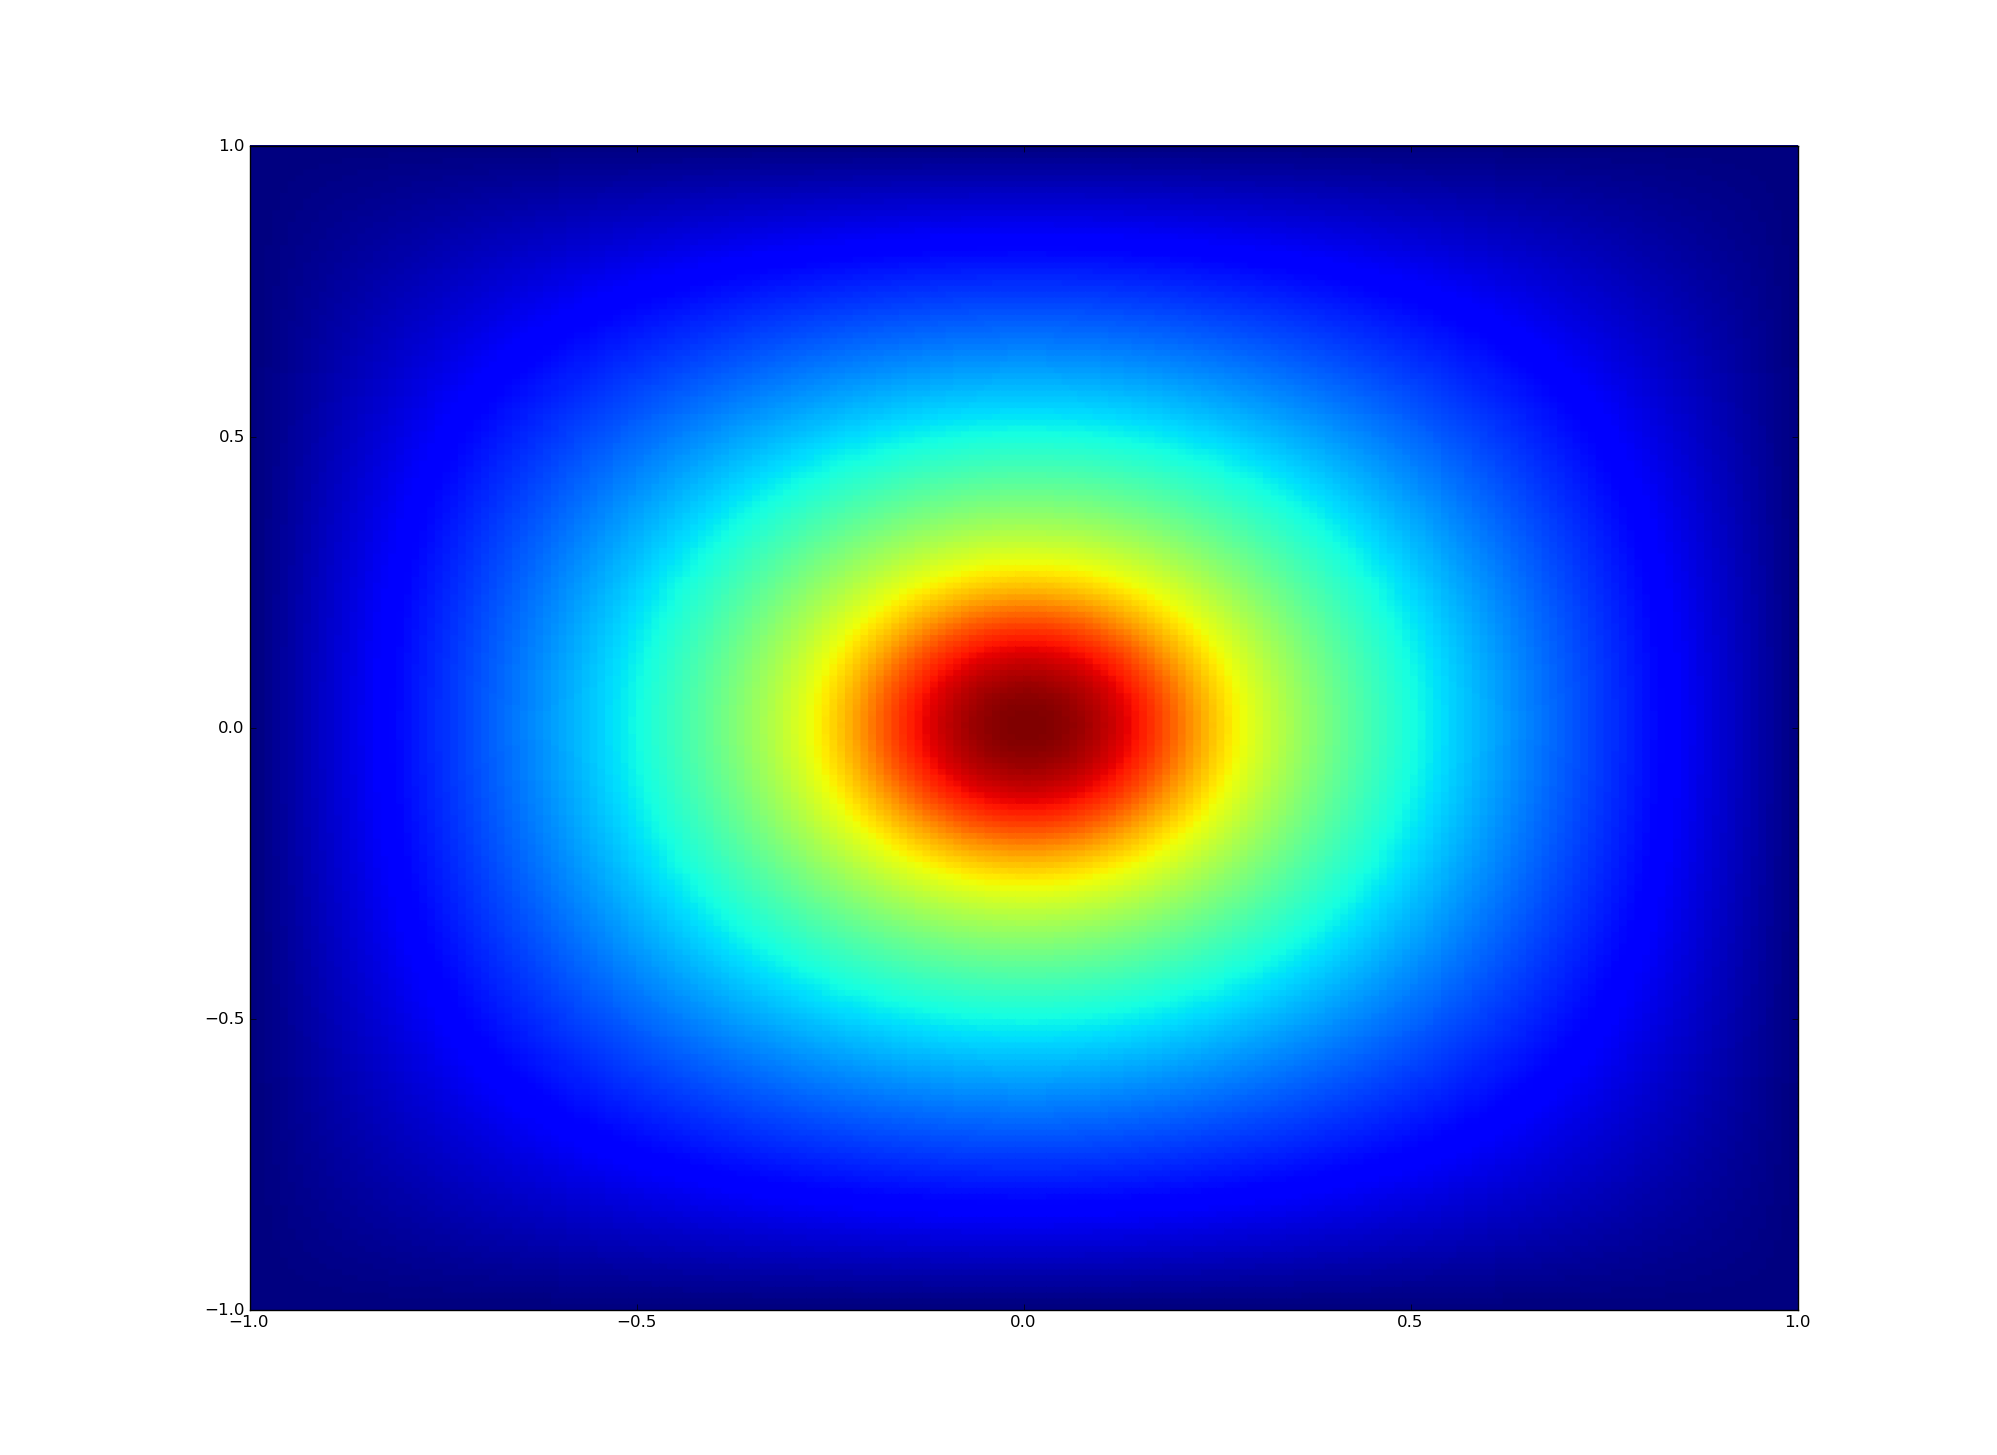
\includegraphics[width=5in]{prob1_result.png}
\end{center}

\paragraph{2}

Since I am using python, I couldn't get the meshgen code to work.  Instead, I downloaded a generic wrapper for QHull and wrote my own mesher based on Delaunay triangulation with a few refinements.  First, the condition that points stay within the set is rewritten as a single unilateral constraint, which can be achieved using R-functions.  Similarly, the points near the boundary can be clamped turning this constraint into an optimization problem.  The starting points for the mesh are taken from a uniform grid, and then jittered a bit.  As a post process, any elements with a sufficiently small initial angle are collapsed.  The removal of these bad quality elements is iterated until all elements have an acceptable quality threshold.  Here is the code I wrote:

\lstinputlisting{trimesh.py}

\lstinputlisting{prob2.py}

And here is the resulting mesh:
\begin{center}

\includegraphics[width=5in]{prob2_result.png}
\end{center}

It is not as good as the meshgen results, but given time limitations it is the best I could come up with.

\paragraph{3}
To set up the weak form of the variational problem, it is sufficient to derive the weak form for the Laplacian operator.  Again, the space of test functions are smooth bumps supported on the domain.  As before, the basis coefficients per element are described a linear system.  Without loss of generality, consider a single element with vertices $(x_1, y_1), (x_2, y_2), (x_3, y_3)$.  Let the basis function for vertex $i$ of this element be given by the following affine function:
\[ \varphi^i(x, y) = \alpha^i_1 + \alpha^i_2 x + \alpha^i_3 y \]
Subject to the constraint $\varphi^i(x_j, y_j) = \delta_{i,j}$.  As before, this gives a linear system:
\begin{eqnarray*}
\alpha^i_1 + \alpha^i_2 x_1 + \alpha^i_3 y_1 & = & \delta_{i,1} \\
\alpha^i_1 + \alpha^i_2 x_2 + \alpha^i_3 y_2 & = & \delta_{i,2} \\
\alpha^i_1 + \alpha^i_2 x_3 + \alpha^i_3 y_3 & = & \delta_{i,3}
\end{eqnarray*}
Which we rewrite as a matrix equation, $M \alpha_i = e_i$, and so the coefficients for the $i^{th}$ element are just the $i^{th}$ row of $M^{-1}$.

Now to integrate over the elements, use Barycentric coordinates again.  Define:
\[ J = \left( \begin{array}{cc}
x_2 - x_1 & y_2 - y_1 \\
x_3 - x_1 & y_3 - y_1
\end{array} \right) \]
\[ \mathcal{T}(\lambda_1, \lambda_2) = J \left( \begin{array}{c}
\lambda_1 \\
\lambda_2 \\
\end{array} \right) + \left( \begin{array}{c}
x_1 \\
y_1 \\
\end{array} \right) \]
Though in this case, we must sum over only one triangle.  To determine the x-component of the Laplacian, we do the following:
\begin{eqnarray*}
\int \limits_{\Delta} \varphi^i_{x}(x,y) \varphi^j_{x}(x,y) dx dy 
& = &
	\frac{1}{\det J} \int \limits_0^1 \int \limits_0^{1-\lambda_2}
		\varphi^i_{x}(\mathcal{T}(\lambda_1, \lambda_2)) 
		\varphi^j_{x}(\mathcal{T}(\lambda_1, \lambda_2)) d \lambda_1 d \lambda_2 \\
& = & 
	\frac{1}{\det J} \int \limits_{0}^{1} \int \limits_0^{1 - \lambda_2} 
		\alpha^i_2 \alpha^j_2 d \lambda_1 d \lambda_2 \\
& = & \frac{\alpha^i_2 \alpha^j_2}{2 \det J}
\end{eqnarray*}
And thus the weights for the total Laplacian for element $i$ to $j$ are:
\[ p_2(\varphi^i, \varphi^j) = \frac{\alpha^i_2 \alpha^j_2 + \alpha^i_3 \alpha^j_3}{2 \det J} \]
Using this method, I implemented the following modified element type, which reuses my solver from part 1:

\lstinputlisting{solver2.py}

\lstinputlisting{prob3.py}

Here are some results:
\begin{center}
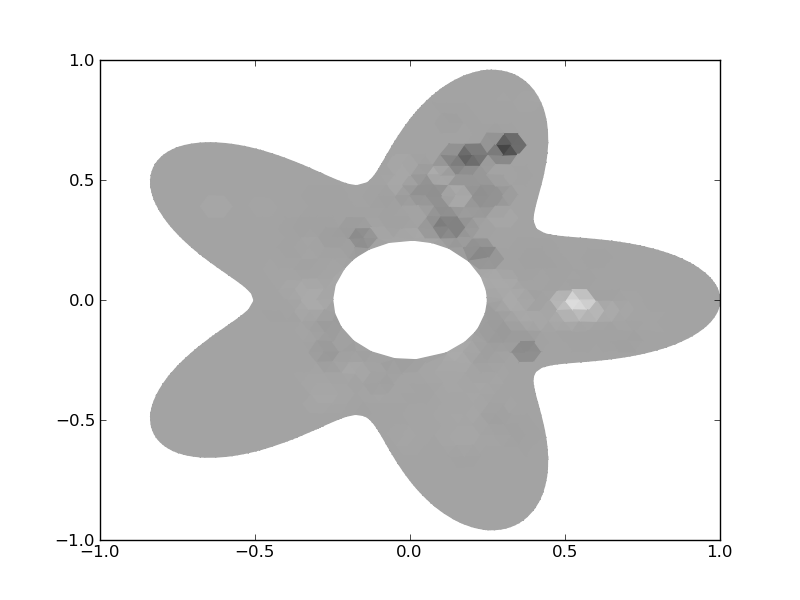
\includegraphics[width=5in]{prob3_result.png}
\end{center}

There appear to be some issues with the set up for the problem.  I would have this working except, I spent too much time trying to get the mesh to draw properly using pylab. I think that given a few more hours I could get this working.

\paragraph{4}

To compute this, we just need to set up the Laplacian matrix for the system then solve for its top 4 eigenvalues.  In theory, the following code should do this:

\lstinputlisting{prob4.py}


But in practice, I get the following eigenvalues:
\[ [ 3.59684369e+09+0.j,  -2.95363663e+09+0.j,   7.68667041e+08+0.j,  -8.05749193e+08+0.j ] \]

And these eigen vectors:
\begin{center}
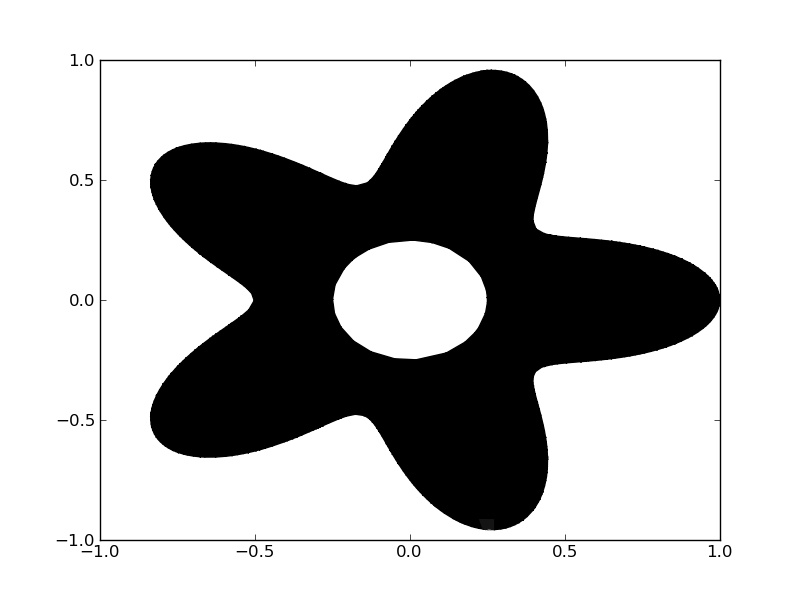
\includegraphics[width=3in]{prob4_eig0.png}

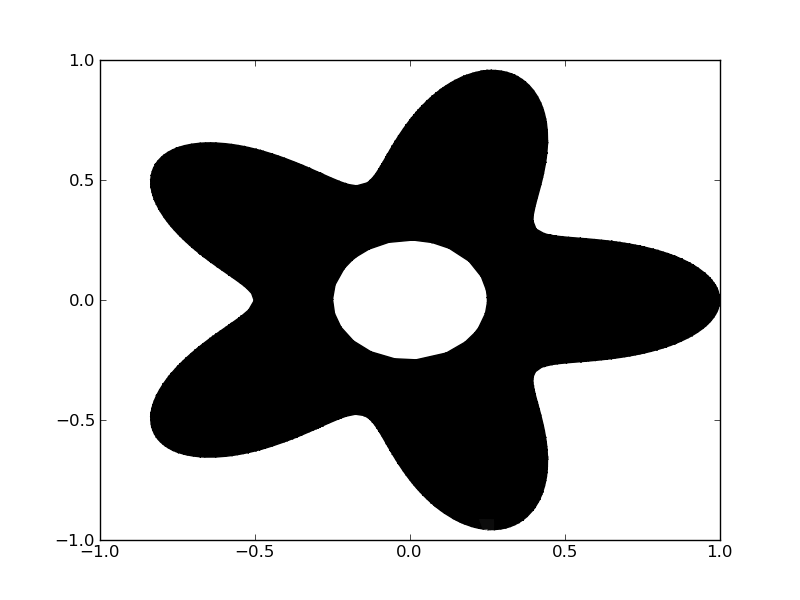
\includegraphics[width=3in]{prob4_eig1.png}

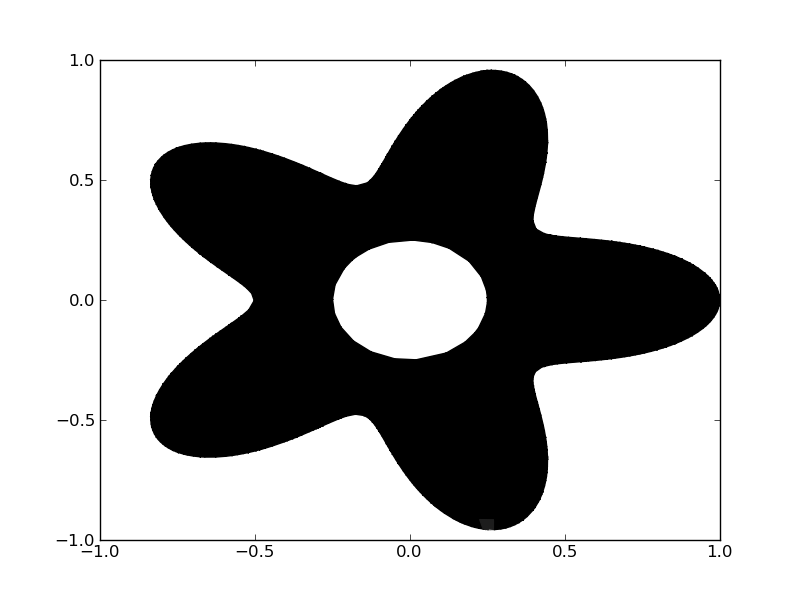
\includegraphics[width=3in]{prob4_eig2.png}

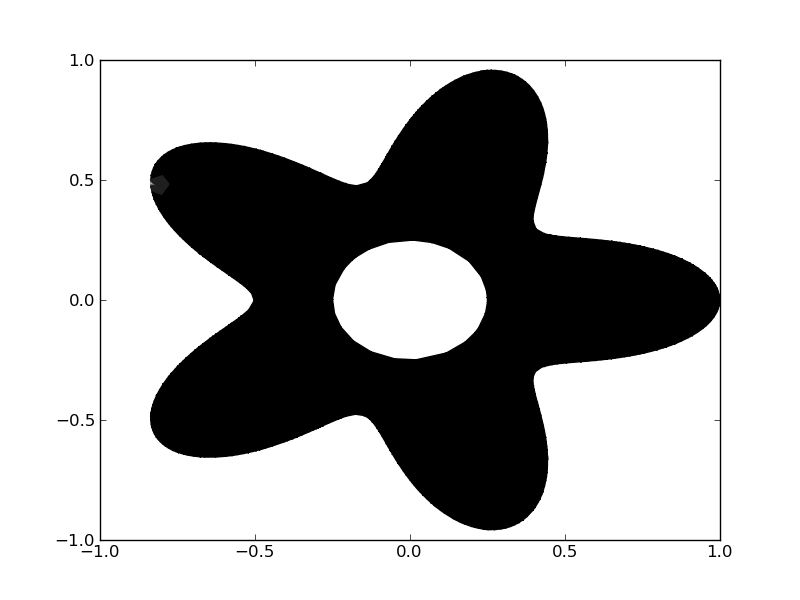
\includegraphics[width=3in]{prob4_eig3.png}
\end{center}

So it seems that I do not have enough time to correct these mistakes.

\end{document}
